\documentclass{standalone}

\usepackage{pgf}
\usepackage{tikz}
\usetikzlibrary{arrows,automata,positioning}
\usepackage[latin1]{inputenc}

\tikzset{every loop/.style={min distance=18mm}}
\tikzset{node distance=2.5cm,
	every state/.style={
		semithick,
		fill=gray!10
	},
	initial text={
		\begin{tabular}{cl}
			5 & $\wedge$ \\
			\hline
			& rcvBase = 1\\
		\end{tabular}},
	double distance=2pt,
	every edge/.style={
		draw,
		->,>=stealth',
		auto,
		semithick
	}
}
\begin{document}
	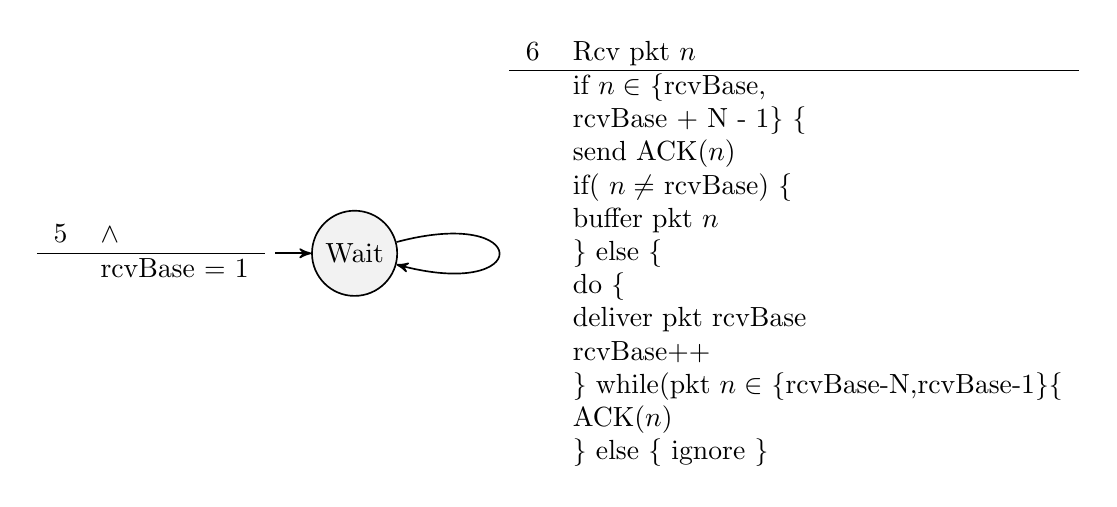
\begin{tikzpicture}
		\node[initial, state] (c) {Wait};
		\draw (c) edge[loop right] node{
			\begin{tabular}{cl}
				6 & Rcv pkt $n$\\
				\hline
				  & if $n \in$ \{rcvBase, \\
				  & rcvBase + N - 1\} \{\\
				  & send ACK($n$)\\
				  & if( $n \neq$ rcvBase) \{\\
				  & buffer pkt $n$ \\
				  & \} else \{ \\
				  & do \{ \\
				  & deliver pkt rcvBase\\
				  & rcvBase++\\
				  & \} while(pkt $n \in$ \{rcvBase-N,rcvBase-1\}\{\\
				  & ACK($n$)\\
				  & \} else \{ ignore \}
			\end{tabular}
		} (c);
	\end{tikzpicture}
\end{document}
